\section{实验结果分析}\label{sec:-2}

本研究获取了合作医院的人类食道的医学造影数据,涉及 4 名患者共计 28 个影像数据。所得数据为患者头颈部侧位DR图像,采用连续采集方式生成视频。图像分辨率为 $480 \times 480$,每个视频的帧数介于 100 至 500 帧之间。

本实验采用 Windows11 操作系统,搭载 AMD R7-3700x @ \SI{3.6}{\giga\hertz} CPU 的个人电脑进行实验评估。代码使用 Python 语言编写,完成了完整的可运行 demo。使用本文方法,处理 $480 \times 480$,400帧规模的DICOM医学影像数据并输出结果,时间消耗约 20 秒。demo 未经多核优化,未使用 GPU,在运行效率上有较大提升空间。

本研究的最终输出结果为视频格式,视频的每一帧图像包括2个子图:原始数据帧图像,以钡餐范围及浓度标定图像。后者以R通道输出,同时取原始图像的20\%亮度作正片叠底。\cref{fig:5_结果1} 和\cref{fig:5_结果2} 是部分数据的输出结果中的截图。
\begin{figure}[!htp]
    \centering
    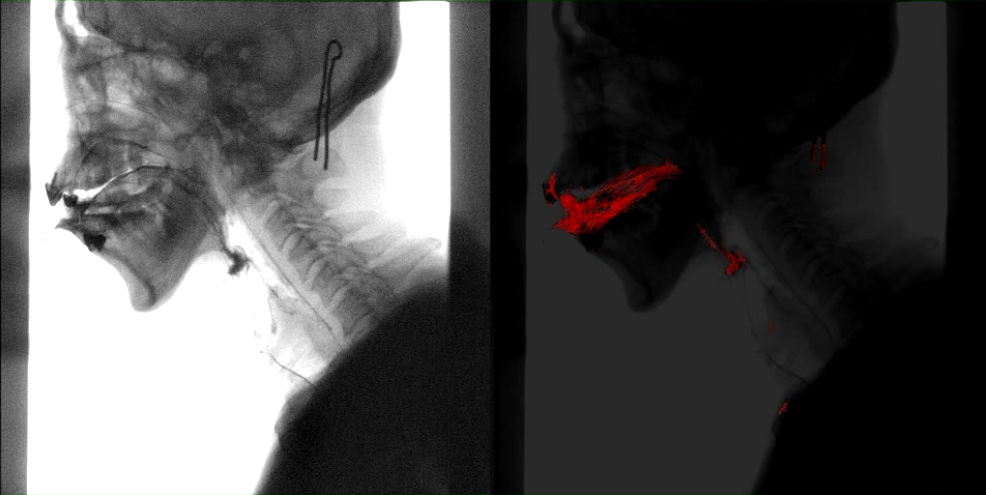
\includegraphics[width=0.8\textwidth]{figures/511.png}
    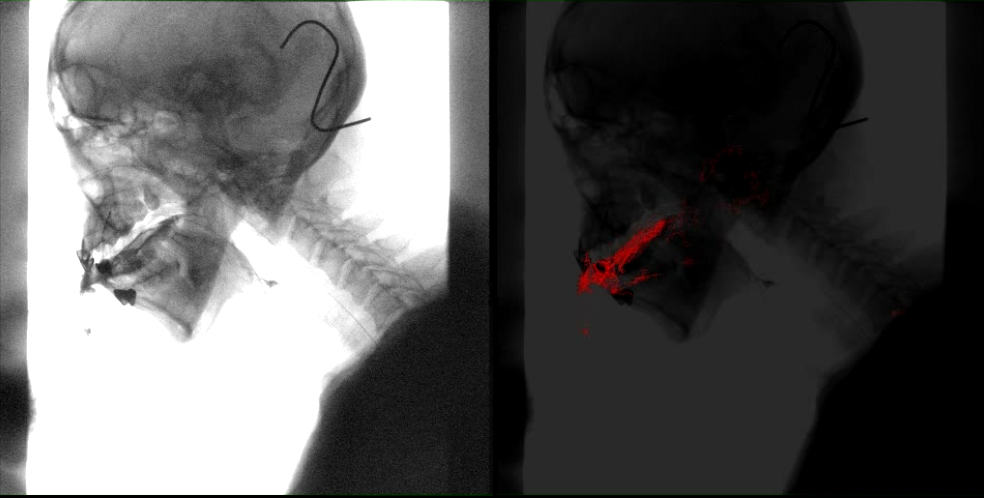
\includegraphics[width=0.8\textwidth]{figures/513.png}
    \caption{钡餐标定结果-口部}
    \label{fig:5_结果1}
\end{figure}

\begin{figure}[!htp]
    \centering
    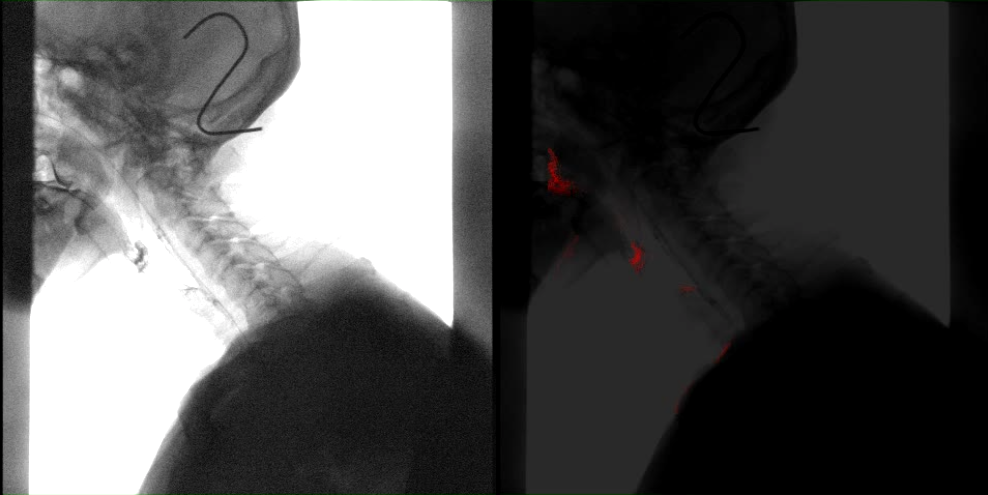
\includegraphics[width=0.8\textwidth]{figures/512.png}
    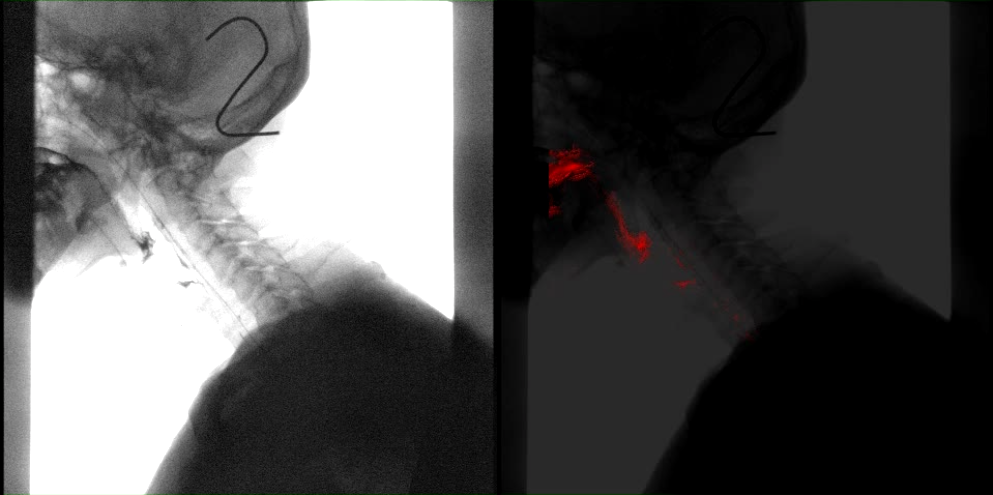
\includegraphics[width=0.8\textwidth]{figures/514.png}
    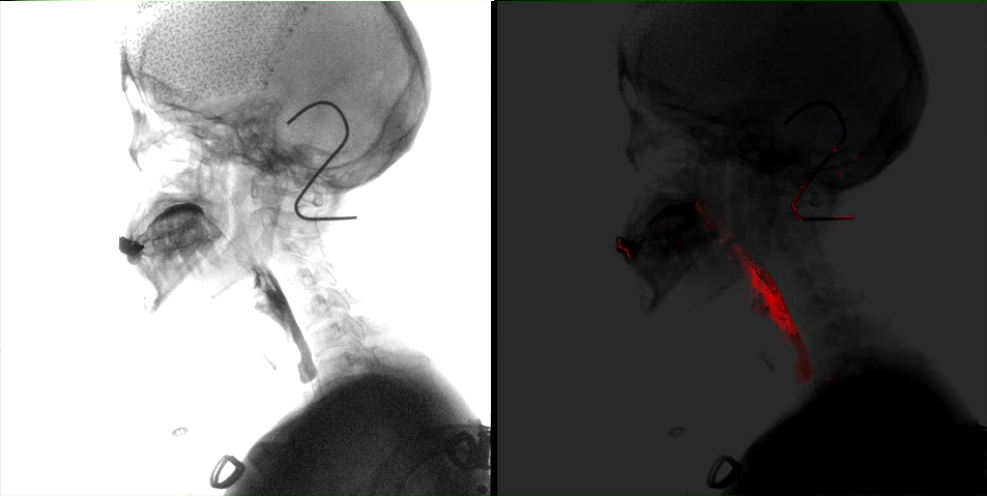
\includegraphics[width=0.8\textwidth]{figures/515.png}
    \caption{钡餐标定结果-喉部}
    \label{fig:5_结果2}
\end{figure}

针对DR图像的分割、标定或三维重建算法的评估,通常会采用相应的MR图像或CT图像作为基准进行对比。然而,本研究涉及的视频数据无法通过这些方法获得。在缺乏更高级设备参考的情况下,通常需要医学专家手动标注以获取标准图像集。然而遗憾的是,本研究仅获得了原始数据,并未获得标准图像集,因此无法通过准确率、精确率、召回率、$F_1$分数或ROC曲线等指标来评估结果。此外,本课题研究内容具备创新性,目前尚未见相关研究或算法模型,暂缺乏与其他方法的结果对比分析。综上,本项目在综合考虑正负样本指标的基础上,采纳了一套以人工观察为主要依据的评价指标。

首先,我们对钡餐在受试者体内各器官的分布情况进行了统计。我们将数据按钡餐在口部出现和在喉部出现分为两类。特别的,若在某组数据中钡餐先后出现在了口部和喉部,我们将该数据的两个副本分别放入两类中。统计表明,钡餐在 82.1\% 的数据中出现在口部,在 60.7\% 的数据中出现在喉部。

接下来,我们对每组数据的处理结果做出评价。评价分为以下类别:
\begin{itemize}
    \item 漏标:存在未被标记的钡餐区域(假阴)。
    \item 多标:不存在漏标,但存在将非钡餐区域标记为钡餐区域(假阳)。
    \item 明显损失:不存在错标,但对钡餐区域的标记存在明显损失,不够完整。
    \item 明显溢出:不存在错标和明显损失,但对钡餐区域的标记存在明显溢出。
    \item 准确:不存在任何以上问题。
\end{itemize}

依照该准则,我们对实验结果进行了评估和统计,详见\cref{tab:5_result}。
\begin{table}[!htbp]
    \centering
    \begin{threeparttable}[b]
        \caption{观察结果}
        \label{tab:5_result}
        \begin{tabular}{@{}lrrrrrrrrrrrrrr@{}}
            \toprule
                & \multicolumn{2}{c}{\textbf{原始数据}} & \multicolumn{2}{c}{\textbf{多标}} & \multicolumn{2}{c}{\textbf{漏标}} & \multicolumn{2}{c}{\textbf{明显溢出}} & \multicolumn{2}{c}{\textbf{明显损失}} & \multicolumn{2}{c}{\textbf{准确}}\\
            \cmidrule(lr){2-3} \cmidrule(lr){4-5} \cmidrule(lr){6-7} \cmidrule(lr){8-9} \cmidrule(lr){10-11} \cmidrule(lr){12-13} \cmidrule(lr){14-15}
                \textbf{器官} & \textbf{数量} & \textbf{占比} & \textbf{数量} & \textbf{占比} & \textbf{数量} & \textbf{占比} & \textbf{数量} & \textbf{占比} & \textbf{数量} & \textbf{占比} & \textbf{数量} & \textbf{占比} \\
            \midrule
                口部            & 25      & 100\% & 7      & 28\% & 1      & 4\% & 8      & 32\% & 1      & 4\% & 8      & 32\%  \\
                喉部            & 17      & 100\% & 0      &  0\% & 0      & 0\% & 8      & 47\% & 1      & 6\% & 8      & 47\%  \\
            \bottomrule
        \end{tabular}
    \end{threeparttable}
\end{table}

分析表中数据可得,本研究的方法应用在喉部数据时尚可,应用于口部数据时欠佳。所有数据的标定结果中,出现漏标和明显损失的占比较少。喉部数据未见错标。错误主要集中在对钡餐区域的标记范围明显溢出,以及口部数据中对非钡餐区域出现了误标。

对于多标错误的数据进行分析发现,有时本文方法会将受试者的后脑勺,患者的衣领,以及护士的袖口等非钡餐区域标记为钡餐区域。这类错误可以通过各种技巧在后处理阶段排除。在实际应用中,这类错误对诊断的影响较小。我们的主要关注点仍然是算法对钡餐在受试者的口、咽、喉部的标定准确度。针对大量数据的标注结果标记范围明显溢出的问题,我们总结了以下原因和改进方案:
\begin{enumerate}
    \item 在行光流法配准时,我们主要以头部轮廓作为配准依据。然而我们观察到,在俯仰动作较大的数据中,头部轮廓的运动矢量和喉管的运动矢量差异巨大,导致配准后的图像中,喉管的位置和实际并不匹配,最终导致标注结果差,在极端情况下,结果甚至不如不进行配准。我们认为一个可行的改进方案为:使用卷积神经网络准确分割出喉管,直接对喉管进行配准。
    \item 我们发现在以下情景中,标注结果会出现明显溢出:护士通过针筒将钡餐注入受试者口腔后,立即用手掌拖住受试者下颌,向上移动下颌来使嘴部闭合,防止钡餐直接流出。此时,嘴部的运动矢量明显大于图像中的其它部位,导致算法将几乎整个嘴部均标记为钡餐区域。我们认为一个可行的改进方案为:对图像进行光流分析时,动态地将图像中“活跃”(即:运动矢量值明显高于整个图像的平均值)的局部提取出来。对该局部单独进行窗宽窗位调整和钡餐区域标定分析。
\end{enumerate}

除此之外,由于本研究主要基于帧间运动信息计算得到最终结果,因此每组影像数据的最初几帧的标注结果通常不够理想。在实验中,钡餐由护士通过针筒注入受试者口腔,应在注射前即开始DR图像的记录。但在实际影像数据中,部分记录始于钡餐已进入受试者口腔后。针对此类数据的标注结果通常出现明显损失甚至漏标。我们认为一个可行的改进方案为:为用户提供一套操作界面,允许研究人员在影像数据的首帧中手动勾画钡餐区域轮廓。在此过程中,可辅以区域生长算法\cite{REVOLMULLER2002137}帮助用户进行标注,根据用户所选坐标点生长出一片标记区域,将轮廓勾画操作简化为多次点选与微调。    

在浓度的标定方面,由于原始采集仪器数据及环境数据暂缺,无法确定钡餐的绝对浓度。在获取原始采集仪器数据及环境数据后,可以根据相关公式计算出绝对浓度值标定。同时还需获取专家的标定结果,方可得到进一步的评价指标,包括:钡餐范围与实际范围重合度、钡餐标定浓度与实际浓度平均方差等。
